\documentclass[11pt, oneside]{article}   	% use "amsart" instead of "article" for AMSLaTeX format
\usepackage{geometry}                		% See geometry.pdf to learn the layout options. There are lots.
\geometry{letterpaper}                   		% ... or a4paper or a5paper or ... 
%\geometry{landscape}                		% Activate for for rotated page geometry
%\usepackage[parfill]{parskip}    		% Activate to begin paragraphs with an empty line rather than an indent
\usepackage{graphicx}				% Use pdf, png, jpg, or eps� with pdflatex; use eps in DVI mode
								% TeX will automatically convert eps --> pdf in pdflatex		
\usepackage{amssymb}
\usepackage{amsmath}
\usepackage{parskip}
\usepackage{color}
\usepackage{hyperref}

\title{Hyperbolic trig functions:  inverse}
%\author{The Author}
%\section{}
%\subsection*{}
\date{}							% Activate to display a given date or no date

\graphicspath{{/Users/telliott_admin/Dropbox/Tex/png/}}
% \begin{center} 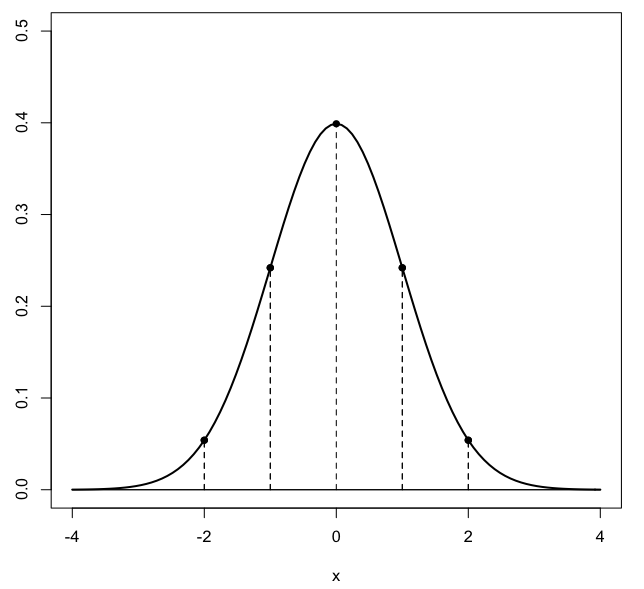
\includegraphics [scale=0.4] {gauss3.png} \end{center}
\begin{document}
\maketitle
\Large
We have looked at the hyperbolic sine and cosine elsewhere:
\[ y = \sinh x = \frac{1}{2} ( e^x - e^{-x} ) \]
\[ y = \cosh x = \frac{1}{2} ( e^x + e^{-x} ) \]
In many ways these are similar to sine and cosine with a sign difference.  For example
\[ \cosh^2 x - \sinh^2 x = 1 \]
\[ \frac{d}{dx} \sinh x = \cosh x \]
\[ \frac{d}{dx} \cosh x = \sinh x \]
Here, our first job is to derive the inverse functions.  To do that we must solve the above equations for $x$.  Take the first one
\subsection*{inverse of sinh}
\[ y = \sinh x = \frac{1}{2} ( e^x - e^{-x} ) \]
\[ x = \sinh^{-1} y \]
Substitute $z=e^x$, then:
\[ 2y = z - \frac{1}{z} \]
\[ z^2 - 2yz -1 = 0 \]
Solve using the quadratic equation
\[ z = \frac{2y \pm \sqrt{4y^2 + 4}}{2} \]
\[ = y \pm \sqrt{y^2 + 1} \]
Since $z = e^x$, $z > 0$ so we take the positive root.  Substitute back to $x$
\[ e^x = y + \sqrt{y^2 + 1} \]
\[ x = \ln | y + \sqrt{y^2 + 1} | \]
Change back to the usual notation with $y$ as the dependent variable
\[ y = \sinh^{-1} x = \ln | x + \sqrt{x^2 + 1} | \]
For the derivative 
\[ \frac{dy}{dx} = \frac{1}{x + \sqrt{x^2 + 1}} \ (1 + \frac{x}{\sqrt{x^2 + 1}} ) \]
\[ = \frac{1}{x + \sqrt{x^2 + 1}} \ (\frac{\sqrt{x^2 + 1} + x}{\sqrt{x^2 + 1}} ) \]
\[ = \frac{1}{\sqrt{x^2 + 1}}  \]
\[ \frac{d}{dx} \sinh^{-1} x = \frac{1}{\sqrt{x^2 + 1}}  \] 
Recall that
\[ \frac{d}{dx} \sin^{-1} x = \frac{1}{\sqrt{1 - x^2}}  \]
Just a change of sign on one term. 
\subsection*{inverse of cosh}
\[ y = \cosh x = \frac{1}{2} ( e^x + e^{-x} ) \]
\[ x = \cosh^{-1} y \]
As before, substitute $z = e^x$
\[ 2y = z + \frac{1}{z} \]
\[ z^2 - 2yz + 1 = 0 \]
\[ z = \frac{2y \pm \sqrt{4y^2 - 4}}{2} \]
\[ = y \pm \sqrt{y^2 - 1} \]
Take the positive root and back substitute
\[ e^x = y + \sqrt{y^2 - 1} \]
\[ x = \ln | y + \sqrt{y^2 - 1} | \]
Change notation:
\[ y = \cosh^{-1} x = \ln | x + \sqrt{x^2 - 1} | \]
Differentiate:
\[ \frac{dy}{dx} = \frac{1}{x + \sqrt{x^2 - 1}} (1 + \frac{x}{\sqrt{x^2 - 1}}  ) \]
\[ = \frac{1}{\sqrt{x^2 - 1}} \]
\[ \frac{d}{dx} \cosh^{-1} x = \frac{1}{\sqrt{x^2 - 1}} \]
Compare with 
\[ \frac{d}{dx} \cos^{-1} x = -\frac{1}{\sqrt{1 - x^2}} \]

\subsection*{inverse of tanh}
Start with 
\[ y = \tanh x = \frac{e^x - e^{-x}}{e^x + e^{-x}} \]
\[ = \frac{e^x - 1/e^x}{e^x + 1/e^x} \]
Substitute $z=e^x$, then:
\[ y = \frac{z - 1/z}{z + 1/z} \]
\[ = \frac{z^2 - 1}{z^2 + 1} \]
\[ (y-1)z^2 + (0)z + (y+1) = 0 \]
The quadratic equation gives:
\[ \frac{\pm \sqrt{-4(y-1)(y+1)}}{2(y-1)} \]
Factor out the $\sqrt{4}$
\[ = \pm \frac{\sqrt{-(y-1)(y+1)}}{(y-1)} \]
\[ = \pm \frac{\sqrt{(1-y)(y+1)}}{(y-1)} \]
Choose the negative root but multiply on the bottom by $-1$
\[ = \frac{\sqrt{(1-y)(y+1)}}{(1-y)} \]
\[ = \frac{\sqrt{y+1}}{\sqrt{1-y}} \]
Substitute back
\[ e^x = \frac{\sqrt{y+1}}{\sqrt{1-y}} \]
\[ x = \ln (\frac{\sqrt{y+1}}{\sqrt{1-y}}) \]
\[ x = \frac{1}{2} \ln (\frac{y+1}{1-y}) \]
Change notation
\[ y = \tanh^{-1} x = \frac{1}{2} \ln (\frac{x+1}{1-x}) \]
Differentiate
\[ \frac{d}{dx} \tanh^{-1} x = (\frac{1}{2}) \frac{1-x}{x+1} \frac{(1-x + x + 1)}{(1-x)^2} \]
\[ = \frac{1-x}{(x+1)(1-x)^2} \]
\[ = \frac{1}{(x+1)(1-x)} \]
\[ = \frac{1}{1-x^2} \]

\end{document}  